\documentclass{article}
\usepackage{amsmath}
\usepackage{amsfonts}
\usepackage{amssymb}
\usepackage{mathdots}
\usepackage{placeins}
\usepackage{relsize,mathtools}
\usepackage{ifthen}
\usepackage{mleftright}
\usepackage{titlesec}
\usepackage{graphicx}
\usepackage{hyperref}
\usepackage[bf]{caption} % For more control over figure captions
\usepackage{subcaption}
\usepackage{listings}
\usepackage{cancel} % term cancellations in math mode
\usepackage{empheq}
\usepackage{tikz} % for drawing vector graphics
\usepackage{float}
\captionsetup{width=\textwidth}
\counterwithin{figure}{section}
\usetikzlibrary{positioning}
\usetikzlibrary{arrows.meta}
\usepackage[top=0.7in, bottom=1in, left=1in, right=1in]{geometry}

\newcommand\E[1]{\left\langle #1 \right\rangle}
\renewcommand{\d}{\mathrm{d}}
\renewcommand\Pr[1]{\begingroup
    \renewcommand\mid{\;|\;}
    \text{P({\larger[2]$\scriptstyle#1$})}
    \endgroup}
\numberwithin{equation}{section}
\hypersetup{
	colorlinks=true,
	linkcolor=blue,
	filecolor=blue,
	urlcolor=blue,
	citecolor=black
}

\begin{document}
\title{Markov chain analysis of overkill and natural regeneration in OSRS combat}
\author{Nukelawe}
\date{\today}
\maketitle

\tableofcontents
\pagebreak

\section{Introduction}\label{chap:introduction}
Most activities in \href{https://oldschool.runescape.com}{Old School RuneScape}~\cite{osrs} are repetitive and feature randomness, making it important to optimize the related expected value quantities. In the case of combat, the subject of optimization is typically either the kill rate or the damage rate (DPS). A method for calculating these quantities is desirable. The main difficulty in these calculations is caused by overkill, which occurs when the enemy does not have enough hitpoints to receive all the damage that was rolled by the attaker. Extra complexity is added by natural regeneration, which affects almost every fight to some, albeit small extent.
Earlier attempts at calculating the kill and damage rates have all made the assumption of no natural regeneration. An approximation for the damage rate was given by~\href{https://imgur.com/aykEahg}{Nukelawe}~\cite{nukelawe} using simplifying assumptions about the long term enemy hitpoint distribution. A more accurate model was presented by \href{https://www.reddit.com/r/2007scape/comments/faz5et/the_mathematics_of_osrs_combat/}{Palfore}~\cite{palfore} and an attempt at an exact solution for the regenerationless case was made by \href{https://www.reddit.com/r/2007scape/comments/bcq3mj/overkill_dps_formulas}{Corpslayer}~\cite{corpslayer1} who also derived an~\href{https://imgur.com/a/6613Tlu}{asymptotic approximation}~\cite{corpslayer2}.

In this study we will drop the assumption of no regeneration and treat Oldschool Runescape fights as absorbing Markov chains. This will allow us to obtain an exact solution for the expected number of hits to kill and the expected number of hitpoints regenerated. From these quantities, we will be able to calculate the kill and damage rates as long time averages. In search of less computationally intensive models and a better understanding of the solution we will additionally study in detail the case of no regeneration as well as some other approximations.

\pagebreak

\section{Fight mechanics}\label{chap:mechanics}
	\subsection{Damage}\label{chap:fightMechanics}
	Consider a scenario in which a single attacker is fighting an unlimited supply of identical passive enemies one at a time. We denote the \textbf{maximum hitpoints} of an enemy by $h$. Once the remaining hitpoints of an enemy reaches 0 the enemy dies and is immediately replaced by a new one with all of its hitpoints remaining. During a fight, the enemy is hit periodically, once every \textbf{attack period} (denoted by $T_A$) and the damage dealt is calulated as follows.
\begin{enumerate}
	\item The game determines if the hit will succeed by some random process, which depends on various parameters such as the defensive bonuses of the enemy, offensive bonuses of the attacker and appropriate combat-related stats. We ignore the details of this process and simply call the probability of success the \textbf{accuracy} (denoted by $a$). If the accuracy check fails, the attack is considered a miss and 0 damage is dealt.
	\item If the accuracy check is successful, damage roll $M\sim U[0,m]$, a uniform random integer between 0 and $m$, is chosen, where $m$ is the \textbf{maximum hit}. Again, we do not concern ourselves with the specifics of how the max hit is determined.
    \item If $M > H$, where $H$ is the remaining hitpoints of the enemy, the damage is capped to $H$ and the final damage dealt is $\min(M,H)$. This is the overkill effect.
\end{enumerate}
Notice that it is possible for the hit to deal no damage even if the accuracy check succeeds because the damage roll $M$ could be 0. For the specifics of max hit and accuracy calculation see for example the \href{https://oldschool.runescape.wiki/w/Maximum_hit}{OSRSwiki articles}~\cite{wiki} on maximum hit and the \href{https://github.com/Palfore/OSRSmath}{OSRS combat overview}~\cite{palfore} by Palfore.

	\subsection{Regeneration}\label{chap:regenMechanics}
	Natural regeneration is a process which periodically attempts to increment the remaining hitpoints by one. A regeneration attempt will fail if the hitpoints are already full. The period $T_R$ of the healing cycle is called the \textbf{regeneration period} and can vary between enemies giving rise to different regeneration rates. At the beginning of a fight the state of the healing cycle can be assumed to be unknown and thus, treated as a uniformly distributed random variable $t_0 \sim U[0,T_R-1]$. This way only the timing of the first regeneration attempt is random and the rest are perfectly periodic.

If measured in \href{https://oldschool.runescape.wiki/w/RuneScape_clock}{ticks}~\cite{wikitick}, the periods $T_A$ and $T_R$ as well as all other quantities that describe time can be assumed integers. We also assume $T_R > T_A$ which ensures that there will be at most one regeneration attempt between any two hits. This assumption should hold for nearly all cases in practice as the the typical regeneration period is 100 ticks (60 seconds) and even the slowest weapons have attack periods of just 7 ticks (4.2 seconds). Another assumption is that the damage dealt by a hit is calculated \emph{after} regeneration if a regeneration attempt occurs on the same tick as the hit. Doing so avoids the edge case in which the enemy dies and then immediately regenerates back to life.

\pagebreak

\section{Markov model}\label{chap:markovModel}
	We define the \textit{state space} as the set of all possible values the remaining hitpoints of the enemy can have during a fight. For a fight against an enemy with $h$ maximum hitpoints this is $\{0,\ldots,h\}$. As each hit corresponds to a transition from one state to another we can think of the fight as a random walk in the state space that terminates in state 0. As an example consider a 4-hitpoint enemy that the attacker hits 3 times: first 1, then 0 and finally 3 damage, killing the enemy. This fight would be described by the sequence $4,3,3,0$ of visited states and corresponds to the highlighted path in the state space diagram in Figure~\ref{fig:stateSpace}.

The probability of transitioning from state $i$ to state $j$ is called the \textit{transition probability} and defined as
\begin{align}\label{eq:transitionProbabilities}
    p_{i,j} = \Pr{H_k = j \mid H_{k-1} = i}
\end{align}
where $H_k$ is the number of hitpoints the enemy has remaining after $k$ hits. The $h+1$ wide square matrix $\mathbf{T}$ that has the transition probabilities as its elements is called the \emph{transition matrix}.
\begin{equation}\label{eq:transitionMatrix}
	\mathbf{T} =
	\begin{pmatrix}
		p_{0,0} & p_{0,1} & \cdots & p_{0,h}\\
		p_{1,0} & p_{1,1} & \cdots & p_{1,h}\\
		\vdots & \vdots & \ddots & \vdots\\
		p_{h,0} & p_{h,1} & \cdots & p_{h,h}\\
	\end{pmatrix}
\end{equation}
The $n$-step transition probability is the probability of transitioning from state $i$ to $j$ in $n$ steps, and we denote it by
\begin{align}\label{eq:nstepTransitionProbabilities}
	p_{i,j}^{(n)} = \Pr{H_k = j \mid H_{k-n} = i}.
\end{align}
It can be read off as the element $i,j$ of the transition matrix power $\mathbf{T}^n$, that is $p_{i,j}^{(n)} = [\mathbf{T}^n]_{i,j}$.
\begin{figure}[h]
    \centering
    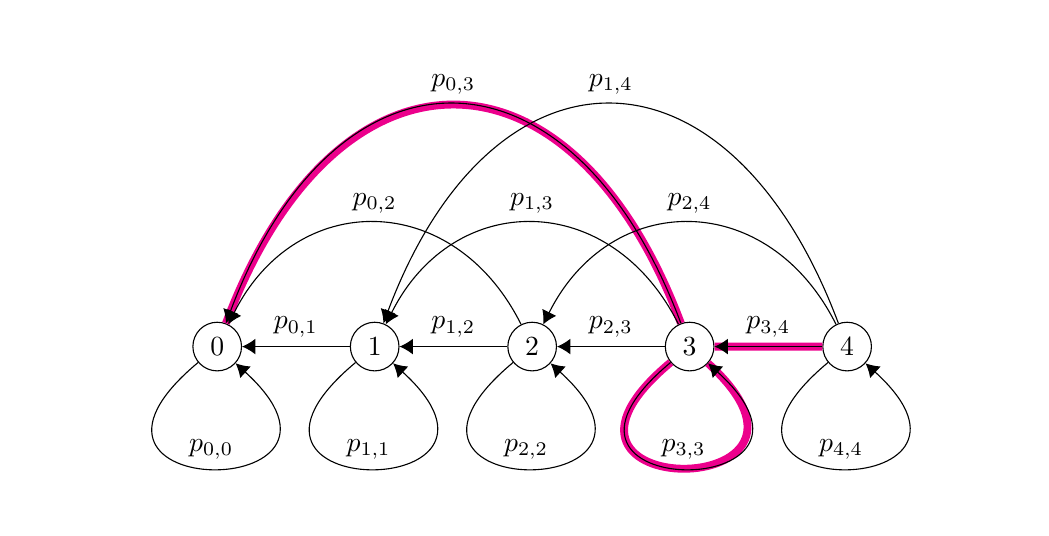
\begin{tikzpicture}[node distance=1cm]
        \tikzstyle{state}=[shape=circle,draw,minimum size=1cm];
        \coordinate (n0);
        \xdef\scale{2}
        \xdef\maxhit{3}
        \foreach \s in {0,1,2,3,4} {
            \node[shape=circle,draw](n\s) at (\scale*\s,0){$\s$};
        }
		\path[draw, color=magenta, line width=1mm] (n4) ..
		controls({(0.75*4+0.25*3)*\scale},{2*(4-3-1)}) and ({(0.25*4+0.75*3)*\scale},{2*(4-3-1)})
		.. (n3) ..
        controls({(3-1.2)*\scale},-2) and ({(3+1.1)*\scale},-2)
		.. (n3) ..
		controls({(0.75*3+0.25*0)*\scale},{2*(3-0-1)}) and ({(0.25*3+0.75*0)*\scale},{2*(3-0-1)})
		.. (n0);
        \foreach \from in {0,1,2,3,4} {
            \foreach \to in {0,1,2,3,4} {
                \foreach \y [evaluate=\y as \yeval using \from-\to] in {1} {
                \foreach \m [evaluate=\m as \meval using int(\to+\maxhit+1)] in {1} {
                    \ifthenelse{\from>\to \AND \from<\meval \AND \to>0}{
						\path[draw,-{Latex[width=2mm]}] (n\from) ..
                        controls({(0.75*\from+0.25*\to)*\scale},{2*(\from-\to-1)}) and ({(0.25*\from+0.75*\to)*\scale},{2*(\from-\to-1)})
                        .. node[above]{$p_{\to,\from}$} (n\to);
                    }{}
                    \ifthenelse{\to=0 \AND \from<\meval \AND \from>0}{
                        \path[draw,-{Latex[width=2mm]}] (n\from) ..
                        controls({(0.75*\from+0.25*\to)*\scale},{2*(\from-\to-1)}) and ({(0.25*\from+0.75*\to)*\scale},{2*(\from-\to-1)})
                        .. node[above]{$p_{\to,\from}$} (n\to);
                    }{}
                    \ifthenelse{\from=\to}{
                        \path[draw,-{Latex[width=2mm]}] (n\from) ..
                        controls({(\to-1.2)*\scale},-2) and ({(\to+1.1)*\scale},-2) .. node[above]{$p_{\to,\from}$} (n\to);
                    }{}
                }
                }
            }
        }
    \end{tikzpicture}\caption{State space diagram for $m=3$, $h=4$ and no regeneration. The probability of moving from state $i$ to $j$ is given with the transition probability $p_{i,j}$. Only edges for which $p_{i,j} > 0$ are shown. The highlighted path corresponds to an example fight.}
	\label{fig:stateSpace}
\end{figure}

	\pagebreak
	\subsection{Transition probabilities}\label{chap:transitionProbabilities}
	Let the accuracy-corrected damage roll $X$ be the damage that would be dealt without considering overkill, or equivalently, on an enemy that had enough hitpoints to receive it. Using the fight mechanics presented in Chapter~\ref{chap:fightMechanics} its probability distribution can be worked out to be
\begin{align}
	\Pr{X=n} = \begin{cases}
		1 - \frac{am}{m+1}, &\mbox{if } n = 0 \\
		\frac{a}{m+1},      &\mbox{if } 1 \leq n \leq m\\
		0,      			&\mbox{if } n < 0\ \mbox{or } m < n
	\end{cases}\label{eq:damageRollDistribution}
\end{align}
where $a$ is the accuracy and $m$ the maximum hit. By also considering overkill we obtain the regenerationless transition probabilities:
\begin{align}
	\pi_{i,j} = \begin{cases}
		\Pr{X = i-j}, &\mbox{if } j > 0 \\
		\Pr{X \geq i-j}, &\mbox{if } j = 0
	\end{cases}\label{eq:noregenTransitionProbabilities}.
\end{align}

When regeneration is considered there are two ways to transition from state $i$ to $j$. To lower the enemy hitpoints by $n$ one can either heal 0 and inflict $n$ damage, or heal 1 and inflict $n+1$ damage. Which one happens depends on whether there is a successful regeneration attempt between the hits. Let $\mathcal{R}_k$ be the event that a regeneration attempt occurs between the $(k-1)$th and the $k$th hits, and denote its complementary event by $\mathcal{R}_k^c$. Remembering that a regeneration attempt will only succeed if the enemy hitpoints are not full or zero we can write the transition probabilities as
\begin{align}
	\Pr{H_k = j \mid H_{k-1} = i} &= \begin{cases}
		\Pr{\mathcal{R}_k}\pi_{i+1,j} + \Pr{\mathcal{R}_k^c}\pi_{i,j},&\mbox{if } 0<i<h\\
		\pi_{i,j},&\mbox{if } i=h\ \mbox{or}\ i=0
	\end{cases}.
\end{align}

To compute the probability $\Pr{\mathcal{R}_k}$ consider the time until the next regeneration attempt immediately after the $k$th hit and denote it by $t_k$. Then $t_0$ is the time until the first regeneration attempt at the beginning of the fight, $T_A$ ticks before the first hit. Since the initial state of the regeneration cycle is assumed to be unknown, $t_0$ is treated as a uniformly distributed random integer $t_0\sim U[0,T_R-1]$. Recall that $t_0$ can only be assumed an integer if $T_R$ is given in ticks (0.6 seconds). The $k$th hit occurs after $kT_A$ ticks from the beginning of the fight. Therefore,
\begin{equation}\label{eq:regenDelay}
	t_k = (t_0 - kT_A) \bmod{T_R}
\end{equation}
which is clearly also uniformly distributed $t_k \sim U[0,T_R-1]$. Now the probability that there is a regeneration attempt between the $(k-1)$th and the $k$th hit is
\begin{align}
	\rho = \Pr{\mathcal{R}_k}
	= \Pr{t_{k-1}\,<\,T_A}
	= \frac{T_A}{T_R}.
\end{align}
This number is called the \emph{regeneration attempt frequency} and can also be interpreted as the probability of regeneration in a model in which regeneration has a chance of occurring between any two hits. Remarkably, it also does not depend on the hit number $k$ at all, making the Markov process time-homogeneous.

In the end, the transition probabilities can be written as
\begin{align}\label{eq:specificTransitionProbabilities}
	p_{i,j} &= \begin{cases}
		\rho\pi_{i+1,j} + (1-\rho)\pi_{i,j},&\mbox{if } 0<i<h\\
		\pi_{i,j},&\mbox{if } i=h\ \mbox{or}\ i=0
	\end{cases}
\end{align}
and the corresponding transition matrix has the form
\begin{align}\label{eq:transitionMatrixShape}
	\mathbf{T} &=
	\begin{pmatrix}
		1 & \mathbf{0} \\
		\mathbf{r} & \mathbf{Q}
	\end{pmatrix}
\end{align}
where $\mathbf{0} = \big(0,\ldots,0\big)$ and $\mathbf{r}$ are a row vector and a column vector of length $h$, respectively, and $\mathbf{Q}$ is an $h$ by $h$ square matrix. Such a transition matrix is characteristic to an absorbing Markov chain. Its $n$th power, the elements of which are the $n$-step transition probabilities, is also easy to compute:
\begin{align}
	\mathbf{T}^n &=
	\begin{pmatrix}
		1 & \mathbf{0} \\
		\big(\mathbf{I}+\mathbf{Q}+\mathbf{Q}^2+\cdots+\mathbf{Q}^n\big)\mathbf{r} & \mathbf{Q}^n
	\end{pmatrix}
\end{align}
By carefully inserting different combinations of states into equation~\ref{eq:specificTransitionProbabilities}, the matrix $\mathbf{Q}$ can be observed to have the following \emph{almost} triangular form.
\setcounter{MaxMatrixCols}{20}
\begin{align}
	\mathbf{Q} =
	\begin{pmatrix}
		p_{1,1} & p_{1,2} & \cdots & p_{1,h}\\
		p_{2,1} & p_{2,2} & \cdots & p_{2,h}\\
		\vdots & \vdots & \ddots & \vdots\\
		p_{h,1} & p_{h,2} & \cdots & p_{h,h}\\
	\end{pmatrix}
	=
	\begin{pmatrix}
		\begin{matrix}
			e_1&e_2\\
			e_3&e_1&e_2\\
			\vdots&\vdots&\vdots&\ddots\\
			e_3&e_3&e_3&\cdots&e_2\\
			e_3&e_3&e_3&\cdots&e_1&e_2\\
			e_4&e_3&e_3&\cdots&e_3&e_1&e_2\\
			   &e_4&e_3&\cdots&e_3&e_3&e_1&e_2\\
			   &   &e_4&\cdots&e_3&e_3&e_3&e_1&e_2\\
			   &   &   &\ddots&\vdots&\vdots&\vdots&\vdots&\vdots&\ddots\\
			   &   &   &      &e_4&e_3&e_3&e_3&e_3&\cdots&e_2\\
			   &   &   &      &   &e_4&e_3&e_3&e_3&\cdots&e_1&e_2
		\end{matrix}\\
		\begin{matrix}
			&&&&&&&&
		\end{matrix}\hspace{39pt}
		\smash[b]{\underbrace{\begin{matrix}
			e_3&e_3&e_3&\cdots&e_3&e_5
		\end{matrix}}_m}
	\end{pmatrix}
\end{align}
where
\begin{align*}
	&e_1 = \frac{\rho a}{m+1} + (1-\rho)\Big(1-\frac{ma}{m+1}\Big)
	&e_2 = \rho\Big(1-\frac{ma}{m+1}\Big)\\
	&e_3 = \frac{a}{m+1}
	&e_4 = (1-\rho)\frac{a}{m+1}\\
	&e_5 = 1-\frac{ma}{m+1}.
\end{align*}

	\subsection{Expected values}\label{chap:expectations}
	\subsubsection{Number of visits}
Let $N_{i,j}$ be the number of times the enemy has $j$ hitpoints during a fight that starts from $i$ hitpoints. The initial state is also counted, so for a fight that starts from full $h$ hitpoints and never regenerates back to $h$, $N_{h,h}$ is the number of zeros hit at the beginning of the fight. We define the indicator function $I_j^k$ such that, $I_j^k = 1$ if the enemy has $j$ hitpoints after the $k$th hit and $0$ otherwise. Now
\begin{align}
	N_{i,j} = \sum_{k\geq 0}I_j^k
\end{align}
and the expected number of visits to state $j$ is
\begin{align}
	\E{N_{i,j}}
	= \E{\sum_{k\geq 0}I_j^k}
	= \sum_{k\geq 0}\E{I_j^k}
	= \E{I_j^0} + \sum_{k\geq 1}\E{I_j^k}
	= \delta_{i,j} + \sum_{k\geq 1}p_{i,j}^{(k)}
\end{align}
where $\delta_{i,j} = 1$ if $i=j$ and 0 if $i\neq j$. Recall that $p_{i,j}^{(k)}$ is the element $i,j$ of the matrix $\mathbf{T}^k$, specifically its transient submatrix $\mathbf{Q}^k$ since we are only considering $i,j > 0$. This allows us to write $\E{N_{i,j}}$ as the element $i,j$ of $\mathbf{I} + \mathbf{Q} + \mathbf{Q}^2 + \cdots$, where $\mathbf{I}$ is the identity matrix of the appropriate shape. Since the enemy will eventually die if hit infinitelly many times, $p_{i,j}^{(k)} \rightarrow 0 \iff \mathbf{Q}^k \rightarrow \mathbf{0}$ as $k \rightarrow \infty$. Therefore the infinite matrix series can, analogously to the regular geometric series, be expressed as
\begin{align}
	\mathbf{I} + \sum_{k\geq 1}\mathbf{Q}^k
	&= {(\mathbf{I} - \mathbf{Q})}^{-1}\nonumber\\
	\implies \E{N_{i,j}} &= \big[{(\mathbf{I} - \mathbf{Q})}^{-1}\big]_{i,j}\label{eq:visitsMatrix}.
\end{align}

\subsubsection{Number of hits to kill}\label{chap:fightLength}
Let a fight's length $L_i$ be the number of hits to kill an enemy that has $i$ hitpoints remaining. Then
\begin{align}
	L_i &= \sum_{j=1}^h N_{i,j}
	\implies \E{L_i} = \sum_{j=1}^h \E{N_{i,j}}.
\end{align}
By defining the $h$-dimensional column vectors $\mathbf{L} = {\big(\E{L_1},\E{L_2},\ldots,\E{L_h}\big)}^T$ and $\mathbf{1} = {(1,1,\ldots,1)}^T$, and using equation~\ref{eq:visitsMatrix} this can be represented as a matrix equation
\begin{gather}
	(\mathbf{I} - \mathbf{Q})\mathbf{L} = \mathbf{1}\label{eq:fightLengthMatrix}
\end{gather}
which is equivalent to a linear system of $h$ equations. The important special case $h=1$ is particularly simple as it is unaffected by regeneration and the system of equations~(\ref{eq:fightLengthMatrix}) reduces to a single equation:
\begin{align}
	(1 - p_{1,1})\E{L_1} &= 1\nonumber\\
	\implies \E{L_1} &= \frac{1}{1 - p_{1,1}}
		= \frac{m+1}{am} \quad\mbox{if }h=1.\label{eq:L1}
\end{align}

\subsubsection{Number of hitpoints regenerated}
The number of hitpoints $R_i$ regenerated during a fight against an enemy with $i$ hitpoints remaining can be obtained by counting the number of successful regeneration attempts. An attempt is successful if the enemy has neither full nor 0 hitpoints at the time the attempt occurs. Let $\mathcal{S}_k$ denote the event that there is a successful regeneration attempt between the $(k-1)$th and the $k$th hits. Then by linearity of expectation
\begin{align}
	\E{R_i}
		&= \sum_{k\geq 0} \Pr{\mathcal{S}_k \mid H_0=i}\nonumber\\
		&= \sum_{k\geq 0} \rho\sum_{j=1}^{h-1} p_{i,j}^{(k)}\nonumber\\
		&= \rho\sum_{j=1}^{h-1}\Big(\delta_{i,j} + \sum_{k\geq 1} p_{i,j}^{(k)}\Big)\nonumber\\
		&= \rho\sum_{j=1}^{h-1}\E{N_{i,j}}\label{eq:regenMatrixDerivation}
\end{align}
Just like we did for $\E{L_i}$, by defining the $h$-dimensional column vectors $\mathbf{R} = {\big(\E{R_1}, \E{R_2}, \ldots, \E{R_h}\big)}^T$ and $\mathbf{1}_h = {(1,1,\ldots,1,0)}^T$, equation~\ref{eq:regenMatrixDerivation} can be expressed in the matrix form
\begin{gather}\label{eq:regenMatrix}
	(\mathbf{I} - \mathbf{Q})\mathbf{R} = \rho\mathbf{1}_h.
\end{gather}

Additionally, from equation~\ref{eq:regenMatrixDerivation} we can derive a handy approximation for $\E{R_h}$. We begin by writing $\E{R_i}$ as
\begin{align}
	\E{R_i}
		&= \rho\sum_{j=1}^{h-1}\E{N_{i,j}}
		= \rho\bigg(\sum_{j=1}^{h}\E{N_{i,j}} - \rho\E{N_{i,h}}\bigg)\nonumber
		= \rho\big(\E{L_i} - \E{N_{i,h}}\big)\label{eq:regenIntuitive}
\end{align}
Assume that the fight starts from full $h$ hitpoints and the damage rate is high enough compared to the regeneration rate, that once left, the state $h$ is never revisited. Then $\E{N_{h,h}}$ can be approximated as the expected number of hits before the state $h$ is left for the first time. This is equal to $\E{L_h}$ in the case when $h=1$, which was calculated to equal $\frac{m+1}{am}$. Therefore,
\begin{align}
	\boxed{\E{R_h}
		\approx \rho\Big(\E{L_h} - \frac{m+1}{am}\Big)
	}
\end{align}

	\subsection{Kill and damage rates}\label{chap:rates}
	Typically the expected values discussed in Chapter~\ref{chap:expectations} themselves are not the quantities of interest. Instead, the aim is often to optimize a rate quantity such as damage per second (DPS) or kills per hour. Such quantities can be easily expressed in terms of the expected values $\E{L}$ and $\E{R}$. Here we have dropped the index $i$ assuming initial state is $h$, i.e. $\E{L} \equiv \E{L_h}$. We will be using the same notation also in the later chapters.

Consider a sequence of $n$ fights against identical enemies. If the length of the $i$th fight in this sequence is denoted by $L_i$ then the time taken by all the fights together is $T_A(L_1+\cdots+L_n)$. Likewise, if the hitpoints regenerated during the $i$th fight is denoted by $R_i$ then the total damage dealt is $nh + R_1+\cdots+R_n$. The \emph{kill rate} and \emph{damage rate} are defined as
\begin{align}
	v_k &= \lim\limits_{n\rightarrow\infty} \frac{n}{T_A(L_1 + \cdots + L_n)}
		= \lim\limits_{n\rightarrow\infty} \frac{1}{T_A\overline{L_n}}\\
	v_d &= \lim\limits_{n\rightarrow\infty} \frac{nh+R_1+\cdots+R_n}{T_A(L_1 + \cdots + L_n)}
		= \lim\limits_{n\rightarrow\infty} \frac{h+\overline{R_n}}{T_A\overline{L_n}}
\end{align}
respectively, where $\overline{L_n} = \frac{1}{n}(L_1+\cdots+L_n)$ is the average number of hits to kill an enemy and $\overline{R_n} = \frac{1}{n}(R_1+\cdots+R_n)$ is the average hitpoints regenerated. Since both $L_i$ and $R_i$ are independent, identically distributed random variables, the law of large numbers implies that $\overline{L_n} \rightarrow \E{L}$ and $\overline{R_n} \rightarrow \E{R}$ as $n\rightarrow\infty$. Hence,
\begin{align}
	\boxed{v_k =
		\frac{1}{T_A\E{L}} \quad\mbox{and}\quad v_d = \frac{h + \E{R}}{T_A\E{L}}.
	}\label{eq:rates}
\end{align}
When $T_A$ is in seconds, $v_d$ is the DPS.

\pagebreak

\section{Approximations}\label{chap:appr}
	In principle, the quantities $\E{L}$ and $\E{R}$ can now be solved from the matrix equations
\begin{gather*}
	(\mathbf{I} - \mathbf{Q})\mathbf{L} = \mathbf{1}
	\quad\mbox{and}\quad
	(\mathbf{I} - \mathbf{Q})\mathbf{R} = \rho\mathbf{1}_h
\end{gather*}
derived in Chapter~\ref{chap:markovModel}. However, doing so requires solving systems of $h$ linear equations, where $h$ is the maximum hitpoints. This can be difficult or slow in practice, especially when $h$ is large. In this chapter we will approximate the Markov process with certain simplifying assumptions.

	\subsection{No regeneration}\label{chap:noregen}
	Let us first assume that there is no regeneration ($\rho = \frac{T_A}{T_R} = 0$), which is a sensible thing to do since most of the time $T_A \ll T_R$. This reduces the transition matrix into a triangular one making an exact analytic solution using forward substitution possible. The effects of overkill still remain which makes such an approximation interesting.

We begin by restating the regenerationless transition probabilities
\begin{align}
	\pi_{i,j} = \begin{cases}
		\Pr{X = i-j}, &\mbox{if } j > 0 \\
		\Pr{X \geq i-j}, &\mbox{if } j = 0
	\end{cases}
\end{align}
where
\begin{align}
	\Pr{X=n} = \begin{cases}
		1 - \frac{am}{m+1}, &\mbox{if } n = 0 \\
		\frac{a}{m+1},      &\mbox{if } 1 \leq n \leq m\\
		0,      			&\mbox{if } n > m\ \mbox{or } n < 0.
	\end{cases}
\end{align}
Obviously, $\E{R_i} = 0$ because there is no regeneration, so it suffices to find the expected length of a fight $\E{L_i}$. Note that since there is now no way for the remaining hitpoints of the enemy to transition upwards, a fight against an enemy with $i$ hitpoints remaining is equivalent to one against an enemy for which $i$ is the maximum hitpoints. Therefore, we can without loss of generality assume that the initial state is $h$.
The now triangular transition matrix allows solving for $\E{L_i}$ recursively. To do this we write the matrix equation~(\ref{eq:fightLengthMatrix}) explicitly.
\begin{align*}
	\mathbf{1} &= (\mathbf{I} - \mathbf{Q})\mathbf{L}\\
	\implies 1 &= \sum_{j=1}^h(\delta_{h,j} - \pi_{h,j})\E{L_j}\\
		&= (1 - \pi_{h,h})\E{L_h} - \sum_{j=1}^{h-1} \pi_{h,j}\E{L_j}\\
		&= \big(1 - \Pr{X=0}\big)\E{L_h} - \sum_{j=1}^{h-1} \Pr{X=h-j}\E{L_j}\\
		&= \frac{am}{m+1}\E{L_h} - \sum_{j=h-m}^{h-1} \frac{a}{m+1}\E{L_j}\\
	\implies \frac{am}{m+1}\E{L_h}
		&= 1 + \frac{a}{m+1}\sum_{j=h-m}^{h-1} \E{L_j}
\end{align*}
To simplify the summation limits, we have defined $\E{L_i} = 0$ for $i \leq 0$. Finally, after reversing the order of summation and multiplying by $\frac{m+1}{am}$ the recurrence relation becomes
\begin{align}
	\E{L_h} = \E{L_1} + \frac{1}{m}\sum_{j=1}^m \E{L_{h-j}}\label{eq:noregenRecursion}
\end{align}
where $\E{L_1} = \frac{m+1}{am}$ as discussed in Chapter~\ref{chap:fightLength}.

		\subsubsection{Analytic solution}\label{chap:noregenSolution}
		Equation~\ref{eq:noregenRecursion} is a linear recurrence of order $m$ with constant coefficients. It can be solved using a generating function $g(z)$, which when expanded as power series around $z=0$ has $\E{L_h}$ as its coefficients:
\begin{align}
	g(z) = \sum_{h=1}^{\infty} \E{L_h} z^h\label{eq:ogf0}.
\end{align}
The generating function can be found by substituting the recurrence relation in place of $\E{L_h}$ in equation~\ref{eq:ogf0}.
\begin{align}
	g(z)
		&= \sum_{h=1}^\infty\bigg(\frac{m+1}{am} + \frac{1}{m}\sum_{j=1}^m \E{L_{h-j}}\bigg)z^h\nonumber\\
		&= \frac{m+1}{am}\sum_{h=1}^\infty z^h + \frac{1}{m} \sum_{h=1}^\infty\sum_{j=1}^m \E{L_{h-j}} z^h \nonumber\\
		&= \frac{m+1}{am}\sum_{h=1}^\infty z^h + \frac{1}{m} \sum_{j=1}^m\sum_{h=1}^\infty \E{L_h} z^{h+j} \nonumber\\
		&= \frac{1}{m}\bigg(\frac{m+1}{a}\frac{z}{1-z} + \sum_{j=1}^m z^j g(z)\bigg)\nonumber\\
		&= \frac{1}{m}\bigg(\frac{(m+1)z}{a(1-z)} + \frac{z - z^{m+1}}{1-z} g(z)\bigg)\nonumber\\
	\implies m(1-z)g(z) &= \frac{(m+1)z}{a} + \big(z - z^{m+1}\big)g(z)\nonumber\\
	\implies \big(m - mz + z^{m+1} - z\big)g(z) &= \frac{(m+1)z}{a}\nonumber\\
	\implies g(z) &= \frac{(m+1)z}{a\big(m - (m+1)z + z^{m+1}\big)}\label{eq:ogf1}
\end{align}
To read off the explicit formula for $\E{L_h}$ the generating function must be expanded back into a power series. We begin by writing it in the form of a geometric sum.
\begin{align}
	g(z) &= \frac{\frac{m+1}{am}z}{1 - \frac{z}{m}(m+1-z^m)}\nonumber\\
	&= \frac{m+1}{am}z \sum_{n=0}^\infty {\Big(\frac{z}{m}\Big)}^n {\big(m+1-z^m\big)}^n\nonumber\\
	&= \frac{m+1}{am}z \sum_{n=0}^\infty {\Big(\frac{z}{m}\Big)}^n \sum_{k=0}^{n} {(m+1)}^{n-k}{(-1)}^k z^{mk} {n \choose k}\nonumber\\
	&= \frac{1}{a} \sum_{n=0}^\infty \sum_{k=0}^{n} {\Big(\frac{m+1}{m}\Big)}^{n+1} {\Big(\frac{-1}{m+1}\Big)}^k {n \choose k}z^{mk+n+1}\label{eq:ogf2}
\end{align}
$\E{L_h}$ is now the coefficient of the term $z^h$. Inspecting the exponent of $z$ in equation~\ref{eq:ogf2} reveals that for the coefficient of interest the indices $k$ and $n$ must satisfy $h=mk+n+1$. For each $k$ there is exactly one valid $n$, namely $n = h-mk-1$. Therefore, the coefficient of the $h$th order term in the series expansion of $g(z)$ is
\begin{align}
    \E{L_h} &= \frac{1}{a}\sum_{k \in \mathcal{I}} {\Big(\frac{m+1}{m}\Big)}^{h-mk} {\Big(\frac{-1}{m+1}\Big)}^k {h-mk-1 \choose k} \nonumber
\end{align}
where $\mathcal{I}$ is the set of indices $k$ such that
\begin{align*}
    0 \leq k \leq n = h-mk-1
    \iff (m+1)k \leq h-1
    \iff k \leq \frac{h-1}{m+1}.
\end{align*}
Since $k$ must also be an integer the index set becomes $\mathcal{I} = \left\{0,1,\ldots,\left\lfloor{\frac{h-1}{m+1}}\right\rfloor\right\}$ and the explicit solution to the recurrence can be written as
\begin{align}
	\boxed{\E{L}
		= \frac{1}{a}
		\sum_{k=0}^{\left\lfloor{\frac{h-1}{m+1}}\right\rfloor} {\left(\frac{m+1}{m}\right)}^{h-mk} {\left(\frac{-1}{m+1}\right)}^k {h-mk-1 \choose k}
	}\label{eq:explicitL}
\end{align}
where the index $h$ in $\E{L_h}$ has been omitted as the fight is assumed to start from full hitpoints.
For small $h$ equation~\ref{eq:explicitL} simplifies to the geometric sequence. In particular,
\begin{align}
	\E{L}
		= \frac{1}{a}{\left(\frac{m+1}{m}\right)}^h \quad \mbox{if }h \leq m+1.
	\label{eq:geomL}
\end{align}
Note how the accuracy dependency can easily be factored out from equation~\ref{eq:explicitL}. This gives a nice interpretation for $a\E{L}$ as the number of \emph{successful hits}, i.e.~hits that pass the accuracy check.

		\subsubsection{Asymptotic approximation}\label{chap:noregenAsymptotics}
		Equation~\ref{eq:explicitL} can be annoying to work with, especially for large initial hitpoints $h$, so an approximation for the case $h \gg m$ is needed. Intuitively the length of a fight should have linear dependency on hitpoints as $h \rightarrow \infty$. This is because on average we can expect each hit to deal $\frac{am}{2}$ damage and therefore it should take approximately $\frac{2h}{am}$ hits to kill an enemy with $h$ hitpoints. Due to overkill however, the last hit will tend to deal slightly less than $\frac{am}{2}$ damage, introducing a constant correction term to this linear approximation. We will now determine the magnitude of this constant by finding the asymptotic expansion for $\E{L_h}$.

To study the asymptotics we inspect the poles of the generating function which are simply the zeros of its denominator. Factorizing out the $(z-1)$ terms in the denominator allows writing the generating function as
\begin{align}
	g(z)
		= \frac{(m+1)z}{a\big(m - (m+1)z + z^{m+1}\big)}
		= \frac{(m+1)z}{{a(z-1)}^2 Q(z)}
	\quad\mbox{where}\quad Q(z) = \sum_{k=0}^{m-1} (m-k) z^k\label{eq:ogf3}.
\end{align}
It is evident from equation~\ref{eq:ogf3} that the generating function has a second order pole at $z=1$. The other poles $q_k$ are the zeros of the polynomial $Q(z)$ and cannot be found exactly. However, since $Q(z)$ is a polynomial with positive coefficients, the Eneström-Kakeya theorem~\cite{kakeya} can be used to obtain a lower bound
\begin{align}
	|q_k|
		\geq \max\limits_{0\leq k < m} \left(\frac{m-k}{m-(k+1)}\right)
		= \frac{m}{m-1} > 1\label{eq:kakeya}.
\end{align}
Now, assume that for some $k$, $q_k$ is not a simple root and thus has a multiplicity greater than 1. Then also the derivative of the denominator of $g(z)$ must have a zero at $q_k$, that is
\begin{align*}
	(m+1)q_k^m - (m+1) = 0
	\implies q_k^m = 1
	\implies |q_k| = 1.
\end{align*}
This contradicts the lower bound we just found (equation~\ref{eq:kakeya}) implying that the poles $q_k$ are all simple.

Having discussed the properties of its poles we now express the generating function as a partial fraction
\begin{align}
	g(z) &=
		\frac{\alpha}{{(z-1)}^2} + \frac{\beta}{z-1}
		+ \sum_k \frac{\gamma_k}{q_k-z}
	\label{eq:ogf4}
\end{align}
where $\gamma_k$ are complex number constants and
\begin{align}
	\alpha
		&= \lim\limits_{z \rightarrow 1}{(z-1)}^2 g(z)
		 = \lim\limits_{z \rightarrow 1} \frac{(m+1)z}{aQ(z)}
		 = \frac{m+1}{aQ(1)},\label{eq:alphamid}\\
	\beta
		&= \lim\limits_{z \rightarrow 1}\frac{\d}{\d z}\Big({(z-1)}^2 g(z)\Big)
		 = \lim\limits_{z \rightarrow 1} \frac{m+1}{aQ(z)}\left(1 - \frac{zQ'(z)}{Q(z)}\right)
		 = \alpha\left(1 - \frac{Q'(1)}{Q(1)}\right)\label{eq:betamid}.
\end{align}
The values of the polynomial $Q(z)$ and its derivative $Q'(z)$ at $z=1$ evaluate to $Q(1) = \frac{1}{2}m(m+1)$ and $Q'(1) = \frac{1}{6}m(m+1)(m-1)$. Substituting them back into equations~\ref{eq:alphamid} and~\ref{eq:betamid} yields
\begin{align}
	\alpha = \frac{2}{am} \quad
	\beta = \frac{2(4-m)}{3am}.
\end{align}
Inserting $\alpha$ and $\beta$ into equation~\ref{eq:ogf4} and expanding each term as a power series around $z=0$ gives
\begin{align*}
	g(z)
		\nonumber&= \frac{2}{am}\frac{1}{{(1-z)}^2} + \frac{2(m-4)}{3am}\frac{1}{1-z} + \sum_k\frac{\gamma_k}{q_k}\frac{1}{1-\frac{z}{q_k}}\\
		\nonumber&= \frac{2}{am}\sum_{n=0}^\infty (n+1) z^n + \frac{2(m-4)}{3am}\sum_{n=0}^\infty z^n + \sum_k \frac{\gamma_k}{q_k}\sum_{n=0}^\infty \frac{z^n}{q_k^n}\\
		&= \sum_{n=0}^\infty \bigg(\frac{2}{am}\Big(n + \frac{m - 1}{3}\Big) + \sum_k \frac{\gamma_k}{q_k^{n+1}}\bigg) z^n
\end{align*}
Remembering that $\E{L}$ is the coefficient of the $h$th order term in the series expansion of the generating function we get
\begin{align}
	\E{L}\label{eq:asymptotic1}
		= \frac{2}{am}\bigg(h + \frac{m-1}{3} + \sum_k \frac{\gamma_k}{q_k^{h+1}}\bigg)
\end{align}
which is the asymptotic expansion we were looking for. By using the triangle inequality and equation~\ref{eq:kakeya} the last term can be bounded as follows.
\begin{align}
	\bigg|\sum_k \frac{\gamma_k}{q_k^{h+1}}\bigg|
	\leq \sum_k \frac{|\gamma_k|}{|q_k|^{h+1}}
	\leq \sum_k |\gamma_k|{\Big(\frac{m-1}{m}\Big)}^{h+1}
	= {\Big(\frac{m-1}{m}\Big)}^{h+1}\sum_k |\gamma_k|
\end{align}
Since $\sum_k|\gamma_k|$ is just a positive real number, we get $\sum_k \frac{\gamma_k}{q_k^{h+1}} = \mathcal{O}\Big({\big(\frac{m-1}{m}\big)}^h\Big)$. Dropping the exponentially vanishing term yields the asymptotic approximation, which Corpslayer~\cite{corpslayer2} also obtained using a different approach.
\begin{align}
	\boxed{\E{L}
		\sim \frac{2}{am}\Big(h + \frac{m-1}{3}\Big)
	}\label{eq:asymptoticAppr}
\end{align}
Figure~\ref{fig:asymptoticApprComparison} illustrates the quality of the asymptotic approximation for various values of $h$ and $m$.
\begin{figure}[h]
    \includegraphics[scale=1.1]{plots/asymptoticApprComparison.pdf}
	\caption{Magnitude of the relative error term $\frac{1}{\E{L}}\sum_k \gamma_k q_k^{-h-1}$ for various values of maximum hit $m$ and initial hitpoints $h$. As expected, the best accuracy is obtained when $h$ is large compared to $m$. The complex roots $q_k$ cause the asymptotic approximation to oscillate around the exact solution making the error term alternate in sign. The clearly visible lines of smaller error are where the sign flips.}\label{fig:asymptoticApprComparison}
\end{figure}

	\subsection{Effective hitpoints approximation}\label{chap:effhp}
	Effects of regeneration can be added to the no regeneration approximation relatively easily by noticing that a fight against an enemy with $h$ hitpoints is equivalent to one against an enemy with $h+R$ hitpoints and no regeneration, where $R$ is the number of hitpoints regenerated during the fight. Since the expected damage of a hit that does not kill the enemy is $\frac{am}{2}$, the expected number of hits it takes to lower the enemy hitpoints by the extra $R$ hitpoints is approximately $\frac{2R}{am}$. A naive attempt at approximating the effects of regeneration could be to assume that the same holds for the expectation:
\begin{align}
	\E{L} &\approx \E{L'} + \frac{2}{am}\E{R}
\end{align}
where $\E{L'}$ is the length of the fight assuming no regeneration.
Now, applying the approximation $\E{R} \approx \rho\big(\E{L}-\frac{m+1}{am}\big)$ obtained in Chapter~\ref{chap:expectations} allows solving for $\E{L}$ in terms of its regenerationless counterpart $\E{L'}$.
\begin{align*}
	\E{L} &\approx \E{L'} + \frac{2\rho}{am}\Big(\E{L}-\frac{m+1}{am}\Big)\\
	\implies \frac{am-2\rho}{am}\E{L} &\approx \E{L'} - \frac{2\rho}{am}\frac{m+1}{am}
\end{align*}
Multiplying both sides by $\frac{am}{am-2\rho} = \frac{1}{1-\frac{2\rho}{am}}$ gives
\begin{equation}
	\boxed{\E{L} \approx
		\frac{1}{1-\frac{2\rho}{am}}\bigg(\E{L'} - \frac{2\rho(m+1)}{{(am)}^2}\bigg)
	}\label{eq:Leffhp}
\end{equation}
from which the number of hitpoints regenerated can be calculated as
\begin{equation}
	\E{R} \approx \rho\Big(\E{L}-\frac{m+1}{am}\Big)\label{eq:Reffhp}.
\end{equation}

As a sanity check we note that if there is no regeneration and $\rho=0$, then $\E{L} = \E{L'}$ and $\E{R}=0$ as they should. The quantity $\frac{2\rho}{am}$ that appears in equation~\ref{eq:Leffhp} is called \emph{relative regeneration rate} as it can be understood as the ratio between the rates at which the enemy hitpoints are incremented ($\rho$) and decremented ($\frac{am}{2}$). A relative regeneration rate of 1 means that, on average, the enemy hitpoints stays the same and the only way for death to ever occur is through random fluctuations. In general, we expect the model to only give good results when $\frac{2\rho}{am} \ll 1$. In contrast to the regenerationless case, the accuracy dependency of $\E{L}$ can no longer be factored out, indicating that the number of hits and the number of \emph{successful} hits are no longer trivially related when regeneration is taken into account.

		\subsubsection{Error analysis}
		Let us denote the relative error of quantity $X$ by
\begin{align}
	\delta X = \frac{X - X'}{X},
\end{align}
where the primed variable $X'$ stands for the approximation of $X$. To study how well the effective hitpoints approximation holds in various regions of the parameter space, we will now inspect the relative errors of the kill rate $v_k$ and the damage rate $v_d$. The true values of $\E{L}$ and $\E{R}$ needed for this comparison can be obtained by numerically solving the matrix equations~\ref{eq:fightLengthMatrix} and~\ref{eq:regenMatrix}.

Figure~\ref{fig:mhErrors} shows how the relative errors of the rates $v_k$ and $v_d$ depend on $m$ and $h$ while keeping the other parameters $a$, $T_A$ and $T_R$ constant.
First, we note that for both rates, the error is 0 for $h=1$ because enemies with 1 hitpoint cannot regenerate. In case of the damage rate $v_d$, the error also vanishes when $m=1$ because then there is no overkill and the expected damage per hit never changes no matter how long the fight lasts or how many hitpoints are regenerated.
In the regions in which some error is present, the error is the largest near the origin where both $m$ and $h$ are small. This is particularly convenient since it is precisely in this region where the numerical solution to the exact Markov model is the fastest. There is currently no explanation for why the error seems to be higher on a blob around the main diagonal as well as on the line of slope $\frac{1}{2}$ intersecting the origin.
\begin{figure}[t]
	\centering
    \includegraphics[scale=1]{plots/mhErrors.pdf}
	\caption{Relative errors of the kill rate $v_k$ and the damage rate $v_d$ in the effective hitpoint approximation for various values of maximum hit and enemy hitpoints. The other relevant parameters $T_A=4$, $T_R=100$ and $a=0.5$ are held constant.}\label{fig:mhErrors}
\end{figure}

\begin{figure}[t]
	\centering
	\begin{subfigure}{\textwidth}
		\centering
		\includegraphics[scale=1]{plots/arErrors.pdf}
	\end{subfigure}
	\begin{subfigure}{\textwidth}
		\centering
		\includegraphics[scale=1]{plots/arErrorLabels.pdf}
	\end{subfigure}
	\caption{Relative errors of the kill rate $v_k$ and damage rate $v_d$ in the effective hitpoint approximation as functions of the relative regeneration rate $\frac{2\rho}{am}$. The regeneration period is assumed to be $T_R=100$ in each fight. The parameters $a$, $m$, $h$ and $T_A$ for the fight scenarios were calculated using the \href{https://github.com/Palfore/OSRSmath}{OSRSmath}~\cite{osrsmath} python-library.}\label{fig:arErrors}
\end{figure}
\FloatBarrier
Figure~\ref{fig:arErrors} shows the relative errors of the kill and damage rates against the relative regeneration rate for various enemy and attacker combinations. For simplicity, no boosts of any kind are considered, and the only gear used is a weapon. The errors are all below $1\,\%$ ($10^{-2}$), most even under $0.1\,\%$ ($10^{-3})$. They would in reality only get smaller as more offensive gear and other boosts are added.
The reason why the relative error of the kill rate increases as the relative regeneration rate approaches 1 is that equation~\ref{eq:Leffhp} has a singularity at the point $\frac{2\rho}{am}=1$. However, most of the fight scenarios in Figure~\ref{fig:arErrors} have relative regeneration rates of less than 0.1 placing them far from the singularity. The only examples in which the relative regeneration rate is anywhere near 1 are the ridiculous ones where a player with level 10 attack and strength, equipped with an iron scimitar, is fighting a relatively strong enemy such as a hellhound. It is no surprise that for such fights regeneration is more significant.
\FloatBarrier

	\subsection{On transition matrix triangularization}\label{chap:otherApproximations}
	Finally, we will briefly discuss another approximation for slow regeneration without going into too much detail. The convenience of the no regeneration assumption was ultimately based on the fact that it made the transition matrix triangular. The same can be accomplished by another, weaker assumption than abandoning regeneration altogether. To ensure that the enemy hitpoints never increase, it is enough to assume that a regeneration attempt never coincides with a hit that inflicts 0 damage.

The transition probabilities in this case are
\begin{equation}
	p_{i,j} = \begin{cases}
		\rho\pi_{i+1,j} + (1-\rho)\pi_{i,j},&\mbox{if } 0<j\leq i<h\\
		\pi_{i,j},&\mbox{if } i=h\ \mbox{or}\ i=0\ \mbox{or}\ j>i
	\end{cases}\label{eq:leastTriProbabilities}
\end{equation}
which yields the recurrence relation
\begin{equation}
	\E{L_i} = \frac{1}{m-\rho}\bigg(\frac{m+1}{a} + \sum_{j=1}^m \E{L_{i-j}} + \rho\E{L_{i-m-1}}\bigg)\label{eq:leastTriRecurrence}
\end{equation}
Although solving equation~\ref{eq:leastTriRecurrence} is significantly harder than without regeneration, it can still be done to a certain extent and at the very least it provides a computationally faster way to solve for the effects of regeneration. Just like in the regenerationless case we find that for small $h$ the fight's length follows a geometric progression:
\begin{equation}
	\E{L}
		= \frac{m+1}{am}{\left(\frac{m-\rho+1}{m-\rho}\right)}^{h-1} \quad \mbox{if }h \leq m+1.
	\label{eq:leastTriGeomL}
\end{equation}

The main disadvantage to this approximation is that the effective hitpoints argument is no longer straightforward to make. Combined with a significantly more difficult to solve recurrence relation, this approximation seems less appealing.

\pagebreak

%\section{Results}\label{chap:results}
%	Figure~\ref{fig:mhValues} shows how $\E{L}$, $\E{R}$, $v_k$ and $v_d$ depend on the maximum hit $m$ and enemy hitpoints $h$. The $\E{L}$ plot illustrates the findings in Chapter~\ref{chap:noregenAsymptotics} that the fight's length increases linearly with $h$ and is inversely proportional to $m$. The number of hitpoints $\E{R}$ correlates very well with $\E{L}$, which was to be expected since $\E{R} = \rho(\E{L} + \E{N_{h,h}})$ and $\E{N_{h,h}}$, the number of times state $h$ is visited, is relatively small for slow regeneration rates. Likewise, the kill rate is simply the inverse of $\E{L}$, so its values are not particularly interesting.
Definitely the most interesting of the plots in Figure~\ref{fig:mhValues} is the one for the damage rate $v_d$, as it clearly displays the region in which the effects of overkill are the most prominent. At low hitpoints increasing the maximum hit barely affects the damage rate, but as the enemy hitpoints increase the effects of overkill vanish and the max hit dependency becomes linear.
\begin{figure}[h]
	\centering
    \includegraphics[scale=1]{plots/mhValues.pdf}
	\caption{The expected number of hits to kill $\E{L}$, number of hitpoints regenerated $\E{R}$, kill rate $v_k$ and damage rate $v_d$ for various values of max hit and enemy hitpoints. The rates are given using game ticks as units of time. The plots were made using the effective hitpoint approximation (eq\ref{eq:Leffhp}) with parameters $T_A=4$ (unarmed, scimitar, etc.), $T_R=100$ (most common regeneration period) and $a=0.5$.}\label{fig:mhValues}
\end{figure}

Figure~\ref{fig:arValues} shows how $\E{L}$, $\E{R}$, $v_k$ and $v_d$ depend on the relative regeneration rate. As we know from the analysis of the regenerationless case, the length of a fight depends on the accuracy as $\E{L} \propto a^{-1}$ and consequently $v_k,v_d \propto a$. Figure~\ref{fig:arValues} shows that around the critical point $\frac{2\rho}{am} = 1$ this relation breaks down. When the regeneration rate is larger than damage rate, $\frac{2\rho}{am} = 1$ and the accuracy dependency satisfies a power law $v_k \propto a^r$, where $r$ is some constant that depends on $m$ and $h$. A particularly violent increase in the fight's length is observed for the curve $m=3$, $h=50$, since now it takes multiple successful lucky hits in succession to lower the enemy hitpoints to 0 before regeneration brings them back up.
In the case $m=50$, $h=3$, we see a deflection \emph{downwards} in the slope of $\E{R}$. Around the critical point this corresponds to a fight in which the accuracy is terrible, but when a successful hit occurs, it inflicts a lot of damage killing the enemy with a high probability. As the accuracy decreases (towards right), such a fight will spend an increasingly large proportion of its duration in the fully regenerated state.
\begin{figure}[h]
	\centering
    \includegraphics[scale=1]{plots/arValues.pdf}
	\caption{$\E{L}$, $\E{R}$, $v_k$ and $v_d$ plotted against the relative regeneration rate $\frac{2\rho}{am}$. For each curve $T_A=4$, $T_R=100$, $m$ and $h$ were held constant while the accuracy $a$ was varied between 0 and 1 to obtain different relative regeneration rates. The curve cutoff point is where $a=1$.}\label{fig:arValues}
\end{figure}

%\pagebreak
%
\section{Conclusions}\label{chap:conclusions}
	We described the damage and natural regeneration mechanics in their full generality using an absorbing Markov chain. The quantities $\E{L}$ (number of hits to kill) and $\E{R}$ (number of hitpoints regenerated) were then shown to be solutions to linear systems of as many equations as the enemy has maximum hitpoints. Because solving such linear systems is computationally intensive for enemies with high hitpoints, we derived a variety of approximations, mainly focusing on small regeneration rates.

Treating in detail the special case of no regeneration we were able to get a good understanding of the effects of overkill. We derived an exact analytic solution (equation~\ref{eq:explicitL}) for the number of hits to kill the enemy and also found a convenient asymptotic approximation (equation~\ref{eq:asymptoticAppr}) for when enemy hitpoints is large compared to the attacker maximum hit. By applying the so called effective hitpoints argument, the regenerationless case was then extended to also approximately account for regeneration. For practically all realistic combat scenarios, the relative errors of the resulting effective hitpoints approximation were observed to be well under $1\,\%$, mostly under $0.1\,\%$. A more rigorous application of the effective hitpoints argument is still worth considering in the future as it might produce even better approximations.

We also briefly discussed a less restrictive assumption that still succeeds in triangularizing the transition matrix. However, because the resulting recurrence relations were more cumbersome to handle and the effective hitpoints argument was difficult to apply, we did not pay much attention to this approximation. Future work might focus on this or other ways of triangularizing the transition matrix. Some thought could also be given on generalizing the asymptotic approximation (equation~\ref{eq:asymptoticAppr}) to consider regeneration.

To conclude, we note that the treatment of the relative simple combat mechanics in Oldschool Runescape can be quite involved. There are also plenty of other combat mechanics that could be considered such as fights against multiple enemies at once, fights against enemies that attack back, poison damage and special attacks.



\bibliography{references.bib}
\bibliographystyle{plain}

\end{document}
